\section*{5/8}
  \subsection*{Periods}
    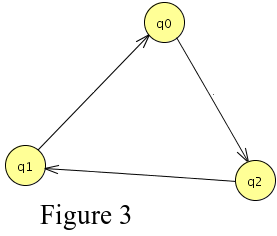
\includegraphics[width=50mm]{5_8_f3.png}
    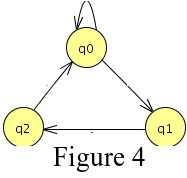
\includegraphics[width=50mm]{5_8_f4.png}\\
    \underline{Example}: Random walk on a undirected square. You have a period of 2.\\
    \underline{Example}: Random walk on a deterministic Chain (figure 3)
      You have a period of 3.\\
    \underline{Example}: Random walk on a undirected triangle. You have a period of 1.\\
    \underline{Example}: Random walk on a deterministic Chain with a chain(figure 4).
      Period is 1.\\
   
   \noindent Let $R_i = \min\{n \ge 1 | X_n = i\}$ or the first time after time 0, that
     the chain is in $i$.\\
     Also, let $f_i^n = P(R_i = n | X_0 = i)$ or the probability that the return time
     to $i$ equals $n$.\\
     Let $f_i = \sum_{n = 1}^{\infty} f_i^n$, which is the $P(\text{ever reenter $i$} |
     X_0 = i)$, so if the chain is recurrent, $\sum_{n = 1}^{\infty}f_i^n = 1$.\\
     \begin{eqnarray*}
      m_i & = & E[R_i | X_0 = i]\\
        & = & \sum_{n = 1}^{\infty} nf_i^n\\
     \end{eqnarray*}
     If $m_i < \infty$, then the series above converges and $i$ is 
     \underline{positive recurrent}.\\
     In this case, the chain is at $i$ every $m_i$ times on average.\\
    \begin{theorem}
      Assume that the chain is irreducible and positive recurrent. Let
      $N_n(i)$ be the number of visits to $i$ in the time interval between
      0 and $n$. Then,
      $$
        \lim_{n \to \infty} \frac{N_n(i)}{n} = \frac{1}{m_i}
      $$
      the former expression is the proportion of time spent at $i$.\\
    \end{theorem}
    \underline{Note}: Very trivial theorem because you need $N_n(i)$ to get
    $m_i$.\\
    \underline{Fact}: Positive recurrent in class property. An irreducible
    chain is positive recurrent if each of its states is. A finite reducible
    chain is always positive recurrent\\
    \begin{theorem}
      An irreducible positive recurrent Markov Chain has a unique 
       \underline{invariant} (aka Stationary distribution. This is a vector
       of possibilities, $\pi_i$ where $i = \{0, 1, 2, \ldots\}$.\\
       $\sum \pi_i = 1$ so that
       $$
        \sum_{\pi_i}P_{ij} = \pi_j \Leftrightarrow [\pi_0, \pi_1, \ldots]
        \cdot = [\pi_0, \pi_1, \ldots]
       $$
       So, $[\pi_0, \pi_1, \ldots]$ is the \underline{left eigenvector} of
       $P$ (for eigenvalue 1). This means that $P(X_0 = i) = \pi_i$ implies
       $P(X_n = i) = \pi_i$. Moreover,
       $$
        \pi_i = \frac{1}{m_i}
       $$
       In fact, an irreducible chain is positive recurrent $\Leftrightarrow$
       a stationary distribution exists.
    \end{theorem}
    \begin{theorem}
      If a Markov Chain is irreducible/aperiodic and positive recurrent, then
      \begin{eqnarray*}
        \lim_{n \to \infty} P_{ij}^n & = & \lim_{n \to \infty} 
          P(X_n = j | X_0 = i)\\
         & = & \pi_j \text{ (no matter what $i$ is)}
      \end{eqnarray*}
    \end{theorem}
    In summary, for finite chains,
    \begin{enumerate}
      \item $\frac{1}{n}N_n(i) \to \pi_i$ $\forall i$
      \item If the chain is aperiodic, 
        $$
          P_{ij}^n \to \pi_j
        $$
        In other words, the matrix $P^n$ eventually looks like
        $$
          \left[
          \begin{array}{c c c c}
            \pi_0 & \pi_1 & \pi_2 & \ldots\\
            \pi_0 & \pi_1 & \pi_2 & \ldots\\
            \vdots & & & \\
          \end{array}
          \right]
        $$
      \item If the chain is aperiodic with period $d$, then
        $\forall i,j$ $\exists r$
        $$
          \lim_{m \to \infty} P_{ij}^{md + r} = d\pi_j
        $$
        For all $n$ such that $n \not= r (\mod d)$,
        $P_{ij}^n = 0$
    \end{enumerate}
  \underline{Example}:
  $$
    P = \left[
    \begin{array}{c c}
      \alpha & 1 - \alpha \\
      \beta & 1 - \beta
    \end{array}
    \right]
  $$
  where $ 0 < \alpha, \beta < 1$
  \begin{enumerate}
    \item 
    $$
      \lim_{n \to \infty} P_{01}^n = \lim_{n \to \infty} 
      P(X_n = 1 | X_0 = 0) = \pi_1
    $$
    \item 
    \begin{eqnarray*}
      \pi_0\alpha + \pi_1 \beta & = & \pi_0\\
      \pi_0(1 - \alpha) + \pi_1(1 - \beta) & = & \pi_1\\
      \pi_0 + \pi_1 & = & 1\\
      &\text{ with a little algebra}&\\
      \pi_0 & = & \frac{\beta}{1 + \beta - \alpha} \\
      \pi_1 & = & \frac{1 - \alpha}{1 - \beta + \alpha}
    \end{eqnarray*}
    \item What is the time spent at 1 if $X_0 = 1$? $\pi_1$
    \item Given $X_0 = 1$, what is the expected return time to 1?
      $\frac{1}{\pi_1}$
    \item Proportion of time the chain is at 1, while the previous 
      time it was at 0? $\pi_0P_{01}$. Look at transitions.
  \end{enumerate}
